\documentclass[compress,mathserif,serif]{beamer}

%\usetheme{Berkeley}

\usepackage{dsfont,calc,xcolor,amsfonts,amsthm,amscd,epsfig,psfrag,amsmath,amssymb,mathtools,commath,enumerate,srcltx,graphicx,xmpmulti}
\usepackage{pgf,tikz}
\usepackage{mathrsfs}
\usetikzlibrary{arrows}
\usetikzlibrary{shapes,backgrounds,positioning,fit}
\usepackage{graphicx}
\usepackage[accumulated]{beamerseminar}

\usepackage{beamerthemeshadow}


\usepackage{pgfpages}
%\setbeameroption{show notes on second screen=left}
%\setbeameroption{previous slide on second screen=left}


\newtheorem{thm}{Theorem}
\newtheorem{Cor}{Corollary}
\newtheorem{question}{Question}
\newtheorem{Con}{Lemma}
\newtheorem{dfn}{Definition}
\newtheorem{proposition}{Proposition}
\newtheorem{remark}{Remark}
\newtheorem{Fact}{Fact}
\newtheorem{conn}{Conjecture}
\newtheorem{rem}{Remark}
\newtheorem{exm}{Example}
\usepackage[english]{babel}


\title[Percolation]{Percolation Theory}
\author[Marco Bertenghi]{\bf Marco Bertenghi}
\institute[UZH]{\bf University of Zurich}


\newcommand{\sref}[1]{SLIDE \ref{#1}}
\setbeamertemplate{navigation symbols}{}
\setbeamertemplate{headline}{}


\usepackage{color}
\usepackage{graphicx}
\usepackage{amssymb}
\usepackage{amsmath}
\usepackage{latexsym}
\usepackage{amsthm}
\usepackage{mathrsfs}
\usepackage{colonequals}


\vspace{4 cm}
\date{}
\vspace{4 cm}

%%%%%%%%%%%%%%%%%%%%%%%%%%%%%%%%%%%%%%%%%%%%%%%%%%%%%
\begin{document}


\begin{frame}
\titlepage
\centerline{\textcolor{blue}{\bf March 19, 2018}}
\vspace{0.5cm}
\end{frame}


\begin{frame}
\frametitle{Motivation}
\begin{itemize}
\item[•] \Large{Understand a simplistic (probabilistic) model for a porous stone. Develop a Toolbox for your daily percolation need.}
\end{itemize}
\end{frame}

\begin{frame}
\tableofcontents
\end{frame}

\section{Framework and Definitions}


\begin{frame}
\begin{center}
\Huge{\color{blue}{\bf{Framework and Definitions}}}
\end{center}
\end{frame}

\begin{frame}
\frametitle{Framework and Definitions}
\begin{itemize}
\item $G=(V,E)$ simple graph.
\pause
\begin{itemize}
\item $V= \mathbb{Z}^d$, $E$ set of edges with $e:=xy$, $x,y \in \mathbb{Z}^d$ that attain unit euclidean distance, i.e. $\| x-y\|_1=1$.
\end{itemize}
\pause
\item Edges are called \textbf{bonds}.
\pause 
\item We let $\mathbb{Z}^d$ refer to the lattice and its vertex set.
\end{itemize}
\end{frame}

\begin{frame}
\frametitle{Framework and Definitions}
\begin{itemize}
\item $\Omega = \{0,1\}^E$ state space.
\pause
\item \textbf{Percolation configuration:}
\begin{itemize}
\item $\omega(e)=1 \rightsquigarrow e$ is open.
\item $ \omega(e)=0 \rightsquigarrow e$ is closed.
\end{itemize}
\pause
\item $\mathcal{F}$ is $\sigma$-algebra generated by events depending only on finitely many edges. 
\pause
\item \textbf{Percolation measure:} $\mathbb{P}_p(\text{Bernoulli}(p))^{\otimes E}$
\end{itemize}
\end{frame}

\begin{frame}
\frametitle{Framework and Definitions}
\begin{dfn}We declare each bond of the lattice $\mathbb{Z}^d$ to be \textbf{open} with probability $p \in [0,1]$ and \textbf{closed} otherwise (i.e. with probability $q=1-p$). Bonds are open or closed independently of all other bonds. 
\end{dfn}
\end{frame}

\begin{frame}
\frametitle{Framework and Definitions}
\begin{dfn}A \textbf{path} (of length $n$) in $\mathbb{Z}^d$ is a sequence of vertices $(x_1, \dots , x_n)$ such that $(x_i,x_{i+1})$ is a bond of $\mathbb{Z}^d.$ A path is called \textbf{open} if all its edges are open and in this case we say that the path connects $x_0$ with $x_n$. A path is called \textbf{closed} if all its edges are closed.
\end{dfn}
\pause
\begin{rem} In percolation we often care about open paths, because such paths simulate where water can flow. 
\end{rem}
\end{frame}

\begin{frame}
\frametitle{Framework and Definitions}
\begin{dfn}Consider the random subgraph of $\mathbb{Z}^d$ which contains only the open edges of $\mathbb{Z}^d$. The connected components of this graph are called \textbf{open clusters}. We denote $C(x)$ to be the open cluster that contains the vertex $x$. 
\end{dfn}
\pause
\begin{rem} By translation invariance of the lattice and the probability measure, the distribution of $C(x)$ is independent of the choice of $x$. We let $C(0)=C$ be the open cluster that contains the origin. 
\end{rem}
\end{frame}

\begin{frame}
\frametitle{Framework and Definitions}
\begin{dfn} We define the \textbf{percolation probability} $\theta(p)$ as the probability that the origin belongs to an infinite open cluster, i.e. 
\begin{align*}
\theta(p):= \mathbb{P}_p(|C|= \infty)
\end{align*} 
\end{dfn}
\end{frame}


\section{Broadbent-Hammersley Theorem}


\begin{frame}
\begin{center}
\Huge{\color{blue}{\bf{Broadbent-Hammersley Theorem}}}
\end{center}
\end{frame}


\begin{frame}
\frametitle{Broadbent-Hammersley Thm}

\begin{Con}There exists a \textbf{critical value} $p_c=p_c(d)$ such that $\theta(p)=0$ for $p<p_c$ and $\theta(p)>0$ for $p>p_c$. Moreover, the critical value is decreasing w.r.t. the dimension, i.e. $p_c(d+1) \leq p_c(d)$.
\end{Con}
\textit{Proof:} Blackboard
\pause
\begin{rem} The one-dimensional case is not interesting because there we have $p_c=1$.
\end{rem}
\end{frame}

\begin{frame}
\frametitle{Broadbent-Hammersley Thm}
\begin{dfn} The parameter set $p<p_c$ is called the \textbf{sub-critical phase}, the set $p > p_c$ is called the \textbf{supercritical phase}.
\end{dfn}
\end{frame}


\begin{frame}
\frametitle{Broadbent-Hammersley Thm}
\begin{dfn} A \textbf{self-avoiding path} of length $n$ is a sequence of edges $e_1, \dots ,  e_n$ with $e_i \neq e_j$ for $i \neq j$ and such that $e_i$ and $e_{i+1}$ share an endpoint for every $1 \leq i <n$. Let $\sigma(n)$ denote the number of self-avoiding paths in $\mathbb{Z}^d$ of length $n$, we define the \textbf{connective constant} of $\mathbb{Z}^d$ as 
\begin{align*}
\lambda(d) = \lim_{n \to \infty} \sigma(n)^{1/n}.
\end{align*}
\end{dfn}
\end{frame}


\begin{frame}
\frametitle{Broadbent-Hammersley Thm}
\begin{dfn} Let $G$ be a graph, we define its dual $G^*$ as the graph which has as vertices the faces of $G$ and as vertices pairs of faces which are adjacent. 
\end{dfn}
\begin{figure}[hbtp]
\centering
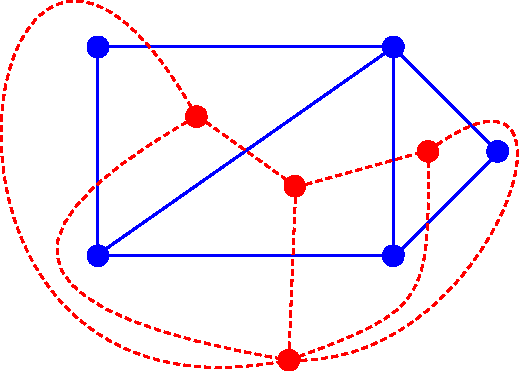
\includegraphics[scale=0.5]{Duals_graphs.pdf}
\caption{The red graph is the dual graph of the blue graph, and vice versa.}
\end{figure}

\end{frame}

\begin{frame}
\frametitle{Broadbent-Hammersley Thm}
\begin{thm}[Broadbent-Hammersley] For $d \geq 2$ we have 
\begin{align*}
0 < \lambda(d)^{-1} \leq p_c(d) \leq p_c(2) <1.
\end{align*}
\end{thm}
\pause
\begin{rem} Later: $p_c(2) \leq (1-\lambda(2)^{-1})).$
\end{rem}
Proof of Theorem: Blackboard.
\end{frame}

\begin{frame}
\frametitle{Broadbent-Hammersley Thm}
\begin{conn}$\theta(p_c)=0$ on $\mathbb{Z}^d$ for every $d \geq 3$.
\end{conn}
\pause
\begin{itemize}
\item Kesten: $p_c(2)=1/2$ and $\theta(p_c)=0$.
\pause
\item Hara and Slade (1990) for $d \geq 19$ (lace expansion).
\pause
\begin{itemize}
\item Lace expansion expected to only work for $d \geq 6$.
\end{itemize}
\pause
\item State of the art: shown for $d \geq 11$.
\end{itemize}
\end{frame}

\section{Harris-FKG inequality}

\begin{frame}
\begin{center}
\Huge{\color{blue}{\bf{Harris-FKG inequality}}}
\end{center}
\end{frame}

\begin{frame}
\frametitle{Harris-FKG}
\begin{dfn} Let $\omega, \omega' \in \Omega$ be two configurations. We say $\omega \leq \omega'$ if $\omega(e) \leq \omega'(e)$ for all bonds $e \in \mathbb{Z}^d$. We say a RV $X: \Omega= \{0,1\}^E \to \mathbb{R}$ is increasing if for $\omega \leq \omega'$ we have $X( \omega) \leq X( \omega')$. An event $A \in \mathcal{A}$ is increasing if $1_A$ is increasing. 
\end{dfn}
\pause
\begin{rem} Heuristically, increasing events are favoured by opening up edges. 
\end{rem}
\end{frame}

\begin{frame}
\frametitle{Harris-FKG}
\begin{exm}The following events are increasing: 
\begin{itemize}
\item $A= \{|C|= \infty\}$ 
\pause
\item $x \longleftrightarrow y$
\pause
\item $B= \{|C_x| \geq 5\}$
\end{itemize}
\pause The following event is neither $\nearrow$ nor $\searrow$:
\begin{itemize}
\item $C= \{|C|=5 \}$.
\end{itemize}
\end{exm}
\end{frame}

\begin{frame}
\frametitle{Harris-FKG}
\textbf{Standard coupling of percolation:}
\begin{itemize}
\item Let $(X_e)_{e \in E}$ be a seq of i.i.d. RV, $X_e \sim \text{unif}[0,1]$.
\begin{itemize}
\item Random label on each edge of percolation model.
\end{itemize}
\pause
\item For all $p \in [0,1]$ we define $\omega_p=(\omega_p(e))_{e \in E}$ by
\begin{align*}
\omega_p(e) = 1_{X_e \leq p }, \text{ for all } e \in E. 
\end{align*}
\end{itemize}
\pause
\begin{proposition}[increasing coupling] Fix $p \leq p'$. There exists a probability measure $\mathbb{P}$ on $[0,1]^E$ which coincides with $\mathbb{P}_p$ on $\{0,1\}^E$ such that $\omega_p \leq \omega_{p'}$ $\mathbb{P}$-a.s.
\end{proposition}
\end{frame}

\begin{frame}
\frametitle{Harris-FGK}
\begin{Con}If $X$ is an increasing RV in $L^1( \mathbb{P}_p) \cap L^1( \mathbb{P}_q)$ then we have \begin{align*}
\mathbb{E}_p(X) \leq \mathbb{E}_q(X), \text{ for } p \leq q. 
\end{align*}
\end{Con}
\pause
\begin{rem} $A= \{|C| = \infty\}$ is increasing $\rightsquigarrow$ $\theta(p)= \mathbb{P}_p(|C|= \infty)$ is increasing. 
\end{rem}
Proof of Lemma: Blackboard.
\end{frame}

\begin{frame}
\frametitle{Harris-FKG}
\begin{thm}[FKG inequality] For increasing random variables $X,Y$ in $L^2( \Omega, \mathbb{P}_p)$, we have
\begin{align*}
\mathbb{E}_p(XY) \geq \mathbb{E}_p(X) \mathbb{E}_p(Y).
\end{align*}
\end{thm}
\pause
\begin{rem} We obtain for positive events $\mathbb{P}_p(A \cap B) \geq \mathbb{P}_p(A) \mathbb{P}_p(B)$ or equivalently $\mathbb{P}_p(A \mid B) \geq \mathbb{P}_p(A)$. 
\end{rem}
Proof of Theorem: Blackboard.
\end{frame}

\begin{frame}
\frametitle{Harris-FKG}
\begin{Cor} We can improve the bound of $p_c(2)$ as follows
\begin{align*}
p_c(2) \leq (1-\lambda(2)^{-1}).
\end{align*}
\end{Cor}
Proof: Blackboard.
\end{frame}

\section{Russo's formula}


\begin{frame}
\begin{center}
\Huge{\color{blue}{\bf{Russo's formula}}}
\end{center}
\end{frame}


\begin{frame}
\frametitle{Russo's formula}
\begin{dfn}Let $A \in \mathcal{A}$ be an event and $\omega \in \Omega$ a configuration. We say that an edge $e \in \mathbb{Z}^d$ is \textbf{pivotal} for the pair $(A, \omega)$ if $1_A(\omega)= 1_A( \widetilde{\omega_e})$ where $\widetilde{\omega_e}$ is the unique configuration which agrees with $\omega$ except at the edge $e$. 
\end{dfn}
\pause
\begin{rem} Pivotal edges are the edges that are essential for an event $A$ to occur. 
\end{rem}
\end{frame}

\begin{frame}
\frametitle{Russo's formula}
\begin{exm} $A=\{|C|= \infty\}$.
\pause
\\
$e$ is pivotal for $A$ iff, when $e$ is removed from the lattice, one endvertex of $e$ is in a finite open cluster containing the origin, the other endvertex is an infinite open cluster.
\end{exm}
\pause
\begin{question} Let $d=2$, how would a pivotal edge for the event $x \longleftrightarrow y$ look like? 
\end{question}
\end{frame}

\begin{frame}
\frametitle{Russo's formula}
\begin{thm}[Russo's formula] Let $A$ be an increasing event, depending only on finitely many edges of $\mathbb{Z}^d$. Then $p \mapsto \mathbb{P}_p(A)$ is differentiable, and 
\begin{align*}
\frac{d}{dp}\mathbb{P}_p(A) = \sum_{e \in F} \mathbb{P}_p(e \text{ is pivotal for } A)
\end{align*}
where $F \subset E$ is a finite subset.
\end{thm}
Proof: Blackboard.
\end{frame}

\section{Exponential decay}


\begin{frame}
\begin{center}
\Huge{\color{blue}{\bf{Exponential decay}}}
\end{center}
\end{frame}

\begin{frame}
\frametitle{Exponential decay}
One major application of Russo's formula is to prove that in the subcritical regime ($p <p_c)$, the connection probabilites decay exponentially fast with distance. 
\pause
\begin{thm}[Exponential decay] For all $d \geq 2$, we have in the subcritical regime $p < p_c$, that there exists a constant $c=c(p)>0$ such that for all $n \geq 1$
\begin{align*}
\mathbb{P}_p( 0 \longleftrightarrow \partial B_n) \leq e^{-cn},
\end{align*}
where $B_n:= \{-n, \dots , n \}^d$ denotes the box of size $n$ around the origin. 
\end{thm}
\end{frame}


\begin{frame}
\begin{center}
\Huge{\color{blue}{\bf{Thank you}}}
\end{center}
\end{frame}


\begin{frame}
\
\end{frame}


\bibliographystyle{unsrt}
\bibliography{biblio}

\end{document}